% =================================
% MSc Report - ROS Integration with ABB 1RB140
% Compiler: latexmk
% =================================
\documentclass[11pt,a4paper]{report}

% -- Core packages --
\usepackage[a4paper,margin=2.5cm]{geometry}
\usepackage[T1]{fontenc}
\usepackage[utf8]{inputenc}
\usepackage{lmodern}
\usepackage{microtype}
\usepackage{titlesec}
\titleformat{\chapter}[hang]{\normalfont\huge\bfseries}{\thechapter}{1em}{}
\titlespacing*{\chapter}{0pt}{-12pt}{18pt}
\usepackage{setspace}
\usepackage{parskip}
\setlength{\parskip}{0.45em}
\usepackage{enumitem}
\setlist[itemize]{itemsep=2pt,topsep=4pt}
\setlist[enumerate]{itemsep=2pt,topsep=4pt}

% -- Headers and footers --
\usepackage{fancyhdr}
\pagestyle{fancy}
\fancyhf{}
\fancyhead[L]{\small\nouppercase{\leftmark}}
\fancyhead[R]{\small Report}
\fancyfoot[C]{\thepage}
\renewcommand{\headrulewidth}{0.4pt}
\setlength{\headheight}{15pt}

% -- Figures, tables and code --
\usepackage{graphicx}
\usepackage{booktabs}
\usepackage{array}
\usepackage{tabularx}
\usepackage{longtable}
\usepackage{float}
\usepackage{needspace}

\usepackage{listings}
\usepackage{etoolbox}
\usepackage{xcolor}
\usepackage{tikz}
\usetikzlibrary{arrows.meta,positioning,fit}

\newcolumntype{Y}{>{\raggedright\arraybackslash}X}
\renewcommand{\arraystretch}{1.15}

% -- Code listing style --
\lstset{
  basicstyle=\ttfamily\small,
  keywordstyle=\color{blue!70!black}\bfseries,
  commentstyle=\color{green!50!black},
  stringstyle=\color{red!60!black},
  backgroundcolor=\color{gray!8},
  frame=single,
  rulecolor=\color{gray!40},
  numbers=left,
  numberstyle=\tiny\color{gray},
  breaklines=true,
  captionpos=b
}

% -- Gantt chart --
\usepackage{pgfgantt}

% -- Bibliography --
\usepackage{cite}

% -- Hyperlinks (load last) --
\usepackage[
  colorlinks=true,
  linkcolor=black,
  citecolor=blue!70!black,
  urlcolor=blue!70!black,
  breaklinks=true,
  pdftitle={ROS Integration with the ABB IRB140 Robotic Platform},
  pdfauthor={Ryan McKee}
]{hyperref}
\usepackage{xurl}

\begin{document}
\setstretch{1.10}
\pagenumbering{gobble}

% -- TITLE PAGE --
\begin{titlepage}
  \thispagestyle{empty}
  \centering
  \vspace*{2cm}

  {\Large \textbf{Department of EEECS}}\\[0.5cm]
  {\large University of Liverpool}\\[3cm]

  {\LARGE \textbf{ROS Integration with the ABB IRB140 Robotic Platform}}\\[1cm]
  {\large MSc Robotics \& IoT -- MSc Final Report}\\[3cm]

  \begin{tabular}{rl}
    \textbf{Author:}     & Ryan McKee \\[4pt]
    \textbf{Student ID:} & 201954749  \\[4pt]
    \textbf{Supervisor:} & Prof.\ Jeremy Smith \\[4pt]
    \textbf{Module:}     & ELEC460 \\[4pt]
    \textbf{Date:}       & \today \\
  \end{tabular}

  \vfill
  {\small Submitted in partial fulfilment of the requirements for the degree of\\ Master of Science in Robotics \& IoT}
\end{titlepage}
\clearpage


\chapter*{Acknowledgements}

\chapter*{Abstract}

This report presents the integration and evaluation of the Robot Operating System
(ROS) with an ABB IRB140 industrial manipulator controlled by an IRB5 controller. A reproducible ROS-Industrial
platform was established using ROS Melodic, abb_driver, a direct Ethernet connection, controller-side motion and state servers 
implemented in ABB's RAPID programming language, and an IRB140 robot description. The resulting system supports live 
joint-state feedback, action-based joint-trajectory commands, MoveIt motion planning, RViz and Foxglove visualization, colour and depth data from an Intel RealSense D405 depth camera,
and rosbag-based experiment recording alongside real life for offline training we developed a digital twin of our robotic cell, mm accurate
world object meshes, added to the world based on exact measurements and ABB IRB140 urdf for loading in gazebo with ROS2 controller for the robotic
arm to mimic the control via IRB140 as well as the design and implementation of a custom pneumatic end effector for the ABB IRB140 to enable 
us to test various simple industrial tasks utilizing the ros integration. we then performed performance analysis of the system 
to see how good it responds to commands etc etc etc. 

\cleardoublepage
\tableofcontents
\cleardoublepage
\phantomsection
\addcontentsline{toc}{chapter}{List of Figures}
\listoffigures
\cleardoublepage
\pagenumbering{arabic}

\chapter{Introduction}

The Robot Operating System \(ROS\) is a widely adopted open-source middleware framework for 
robotic software development. It's modular topic, service and action interfaces allow developers to combine hardware drivers with reusable pakcages for perception, planning, control 
and visualization, why would we be interested in utilizing ROS for this project? there are a few reasons
first the eco system and integration, moveit motion planning library gives a robust trajectory planning and collision avoidance out-of-the-box, extensive sensor integration
makes it easy to integrate my D405 camera within the system, standardized representaition being URDF which allows me to convert cad to urdf

THis is an open-source and research orientated framework, it is community supported and documentation for industrqal arms
reproducibility and transparaency for academic work and gazebo simulation alligns with real system (URDF-based )

middleware benefits include decouples development pipeline for control, enabling distributed processing perception-> planning -> control
standardized message formats for inter-component communication, ABB's official ROS drviers availabel providen in research / industrial settigs, skills transfore to other colllaborative
manipulators (UR, KUKA)


the reason we use ROS1 is because of IRB140 PLATFORM DOES NTO have the egm component in the controller required by the ros2 abb_robot_driver so we utilize 
the older abb_driver which does not have this problem, why don't we use the alternatives, ABB RAPID - navitve programming - tighly coupled to the controller and limits sensor fusion and modulality for vision based sorting task
abb flex pendant gui limited for automated research applications. 

alternative middlewards - Drake ( Toyota robotics library) Excellend for simulation/optimization, but overkill and less alligned with industrial arm drviers
webots/CyberDuck - simulation-frist; not ideal for controlling real hardware
PyBullet - physics engine, not middleware, lacks real-time control abstraction.

OTher robotic platforms include Universal Robots (UR+) OR tECHMAN - they have integrated ecosystems but less open; you're locked 
into their framework
KUKA IIWA or KRL - similar trade-offs to ABB RAPID....


\chapter{Theory Analysis and Design}

\section{End Effector}

\subsection{Requirements}

\subsection{Design}

A two-part design: a tool flange adapter neck, which adds spacing between the tool flange
and the base plate mounting for the components of the end effector.

\begin{figure}[ht]
  \centering
  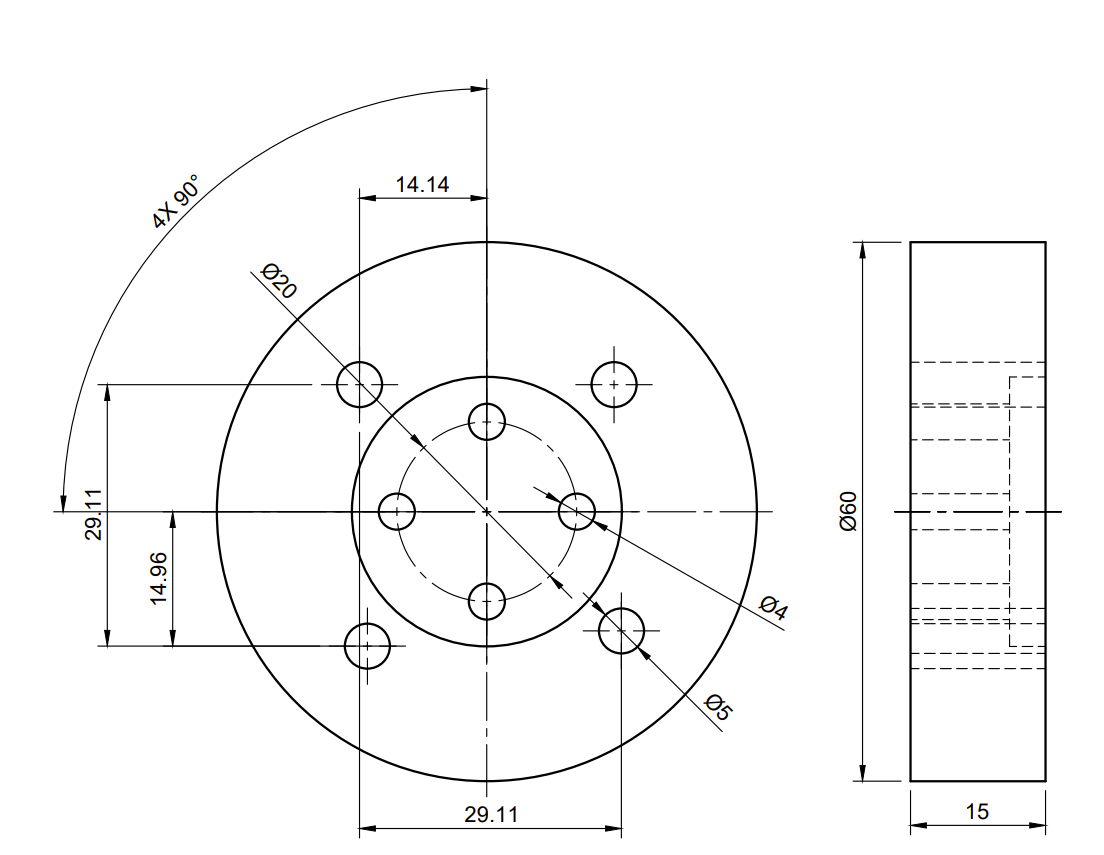
\includegraphics[width=0.7\textwidth]{./figures/design/end_effector_design/flange_adapter_drawing_image.png}
  \caption{End effector tool flange adapter -- drawing}
  \label{fig:flange-adapter-drawing}
\end{figure}

\begin{figure}[ht]
  \centering
  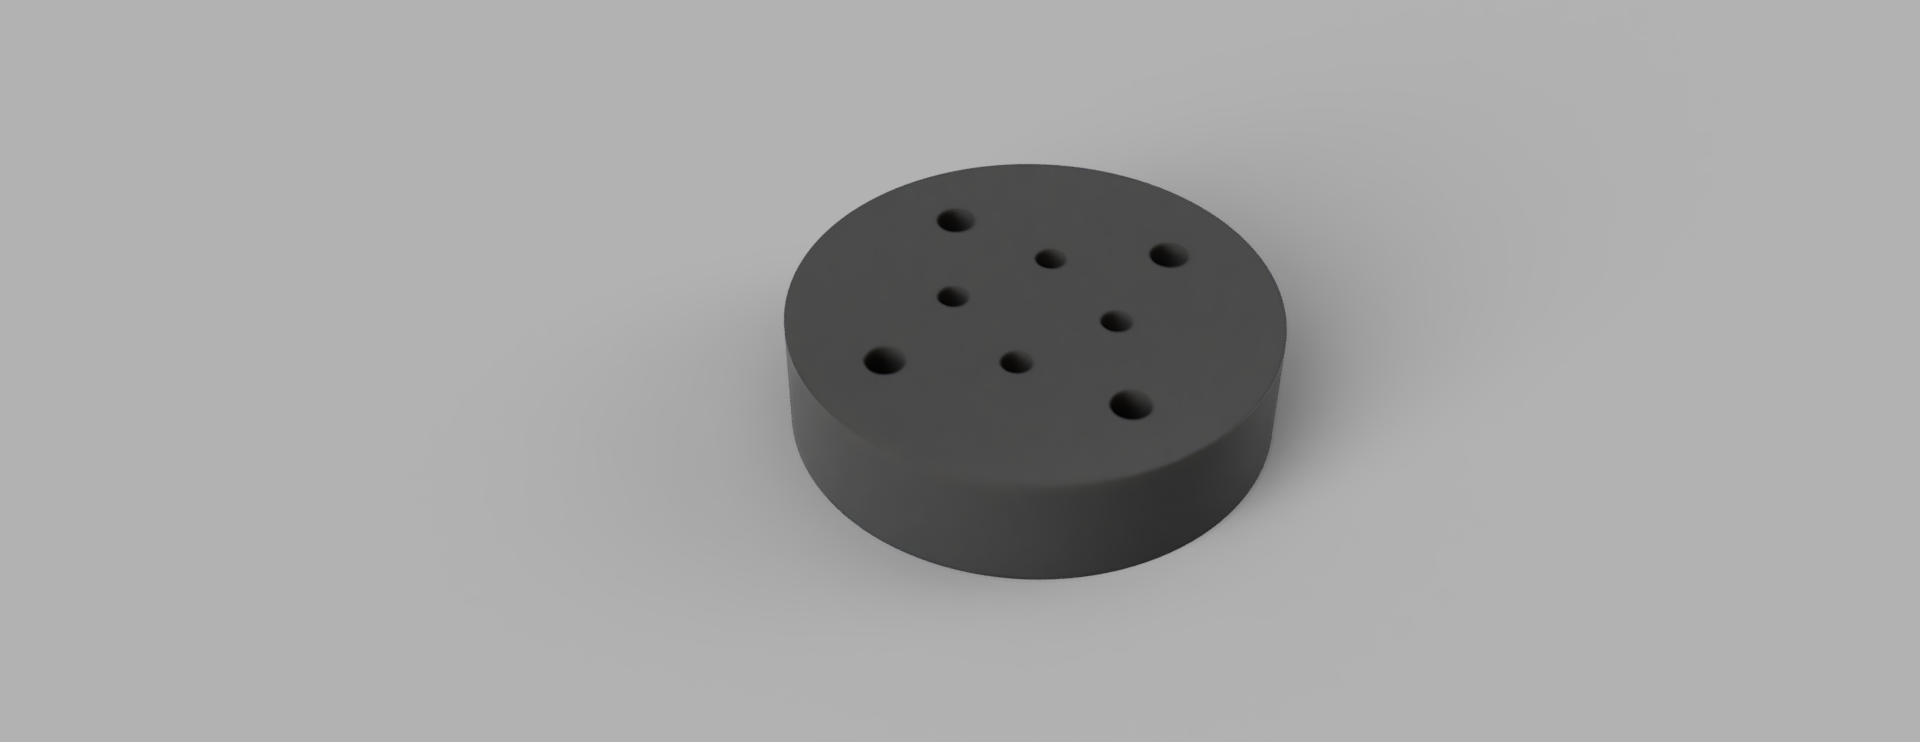
\includegraphics[width=0.7\textwidth]{figures/design/end_effector_design/ABBIRB140_EndEffectBasePlate_2026-Sep-06_12-17-37PM-000_CustomizedView14776947834.png}
  \caption{End effector tool flange adapter -- CAD view}
  \label{fig:flange-adapter-cad}
\end{figure}

\begin{figure}[ht]
  \centering
  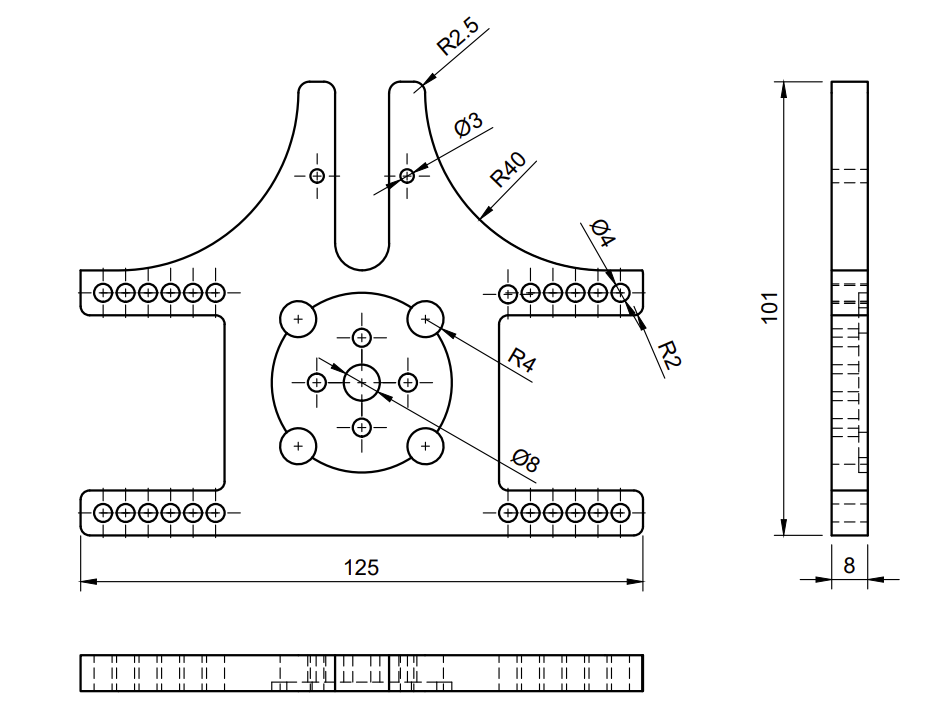
\includegraphics[width=0.7\textwidth]{./figures/design/end_effector_design/end_effector_mounting_plate_drawing_image.png}
  \caption{End effector adapter plate -- drawing}
  \label{fig:adapter-plate-drawing}
\end{figure}

\begin{figure}[ht]
  \centering
  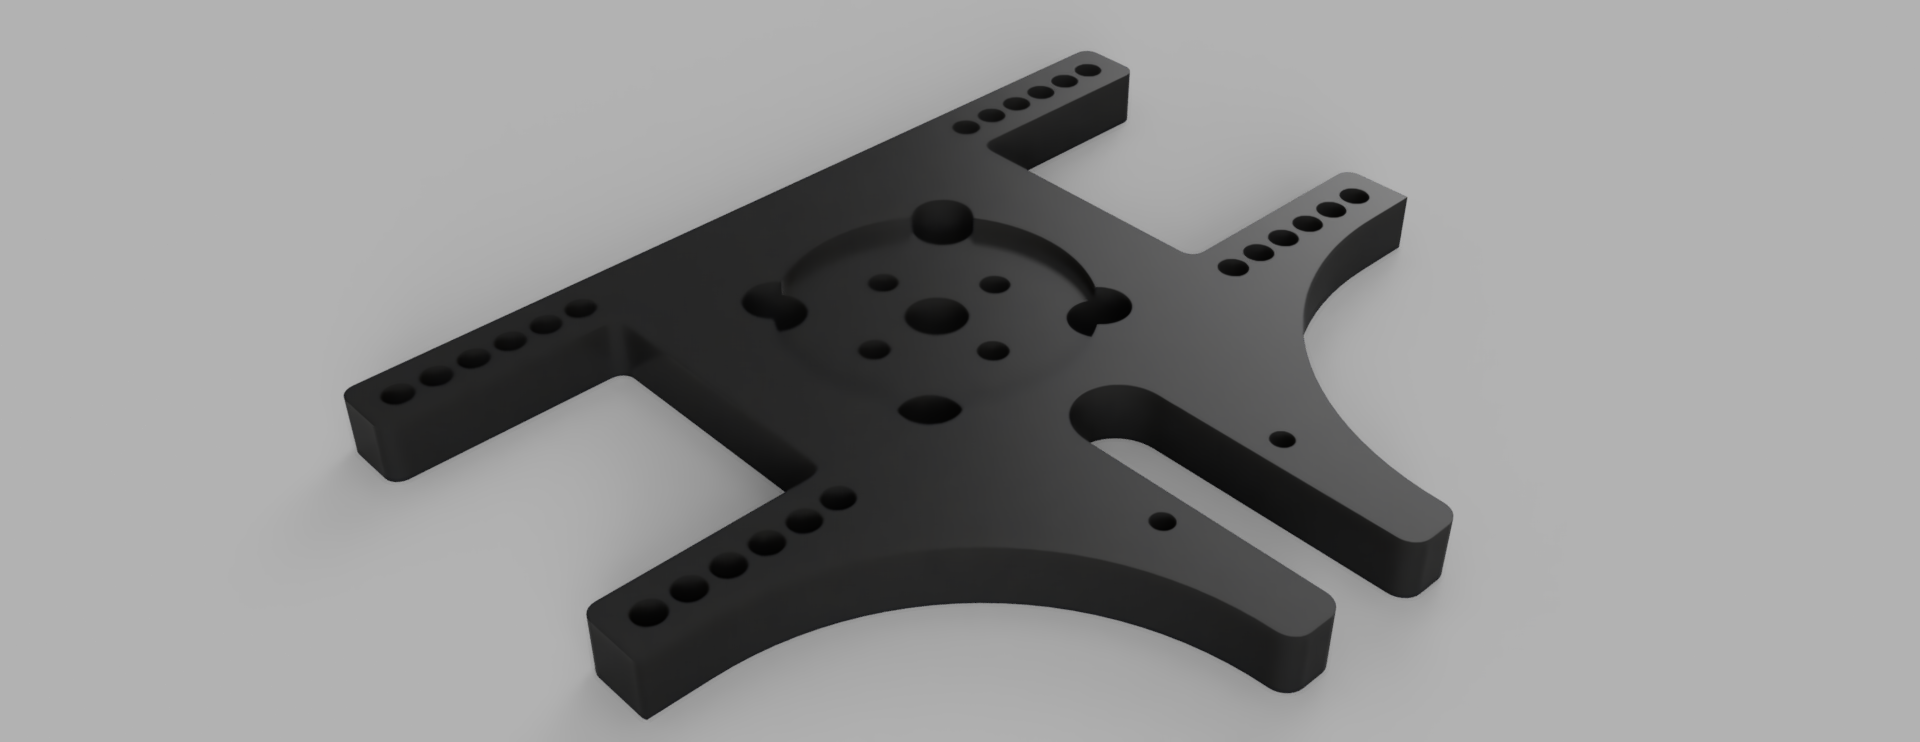
\includegraphics[width=0.7\textwidth]{./figures/design/end_effector_design/end_effector_base_plate_render.PNG}
  \caption{End effector adapter plate -- render}
  \label{fig:adapter-plate-render}
\end{figure}

\begin{figure}[ht]
  \centering
  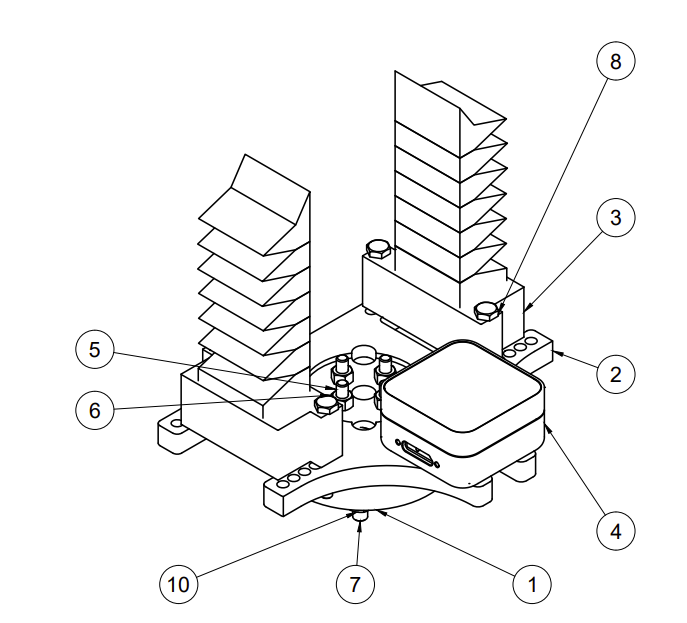
\includegraphics[width=0.7\textwidth]{figures/design/end_effector_design/end_effector_assembly_drawing_image.png}
  \caption{End effector assembly -- drawing}
  \label{fig:assembly-drawing-1}
\end{figure}

\begin{figure}[ht]
  \centering
  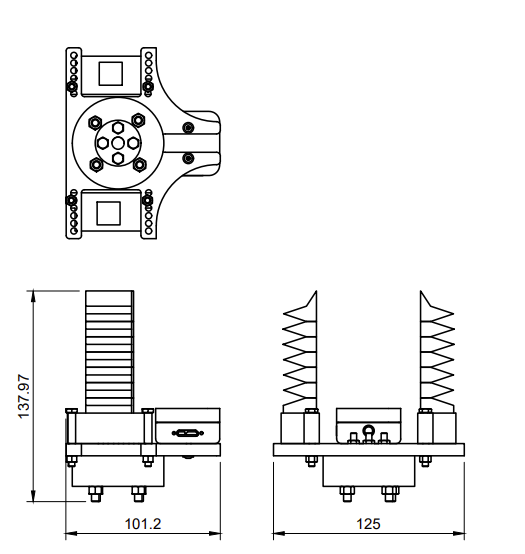
\includegraphics[width=0.7\textwidth]{figures/design/end_effector_design/end_effector_drawing_assembly_image.png}
  \caption{End effector assembly -- drawing, exploded view}
  \label{fig:assembly-drawing-2}
\end{figure}

\begin{figure}[ht]
  \centering
  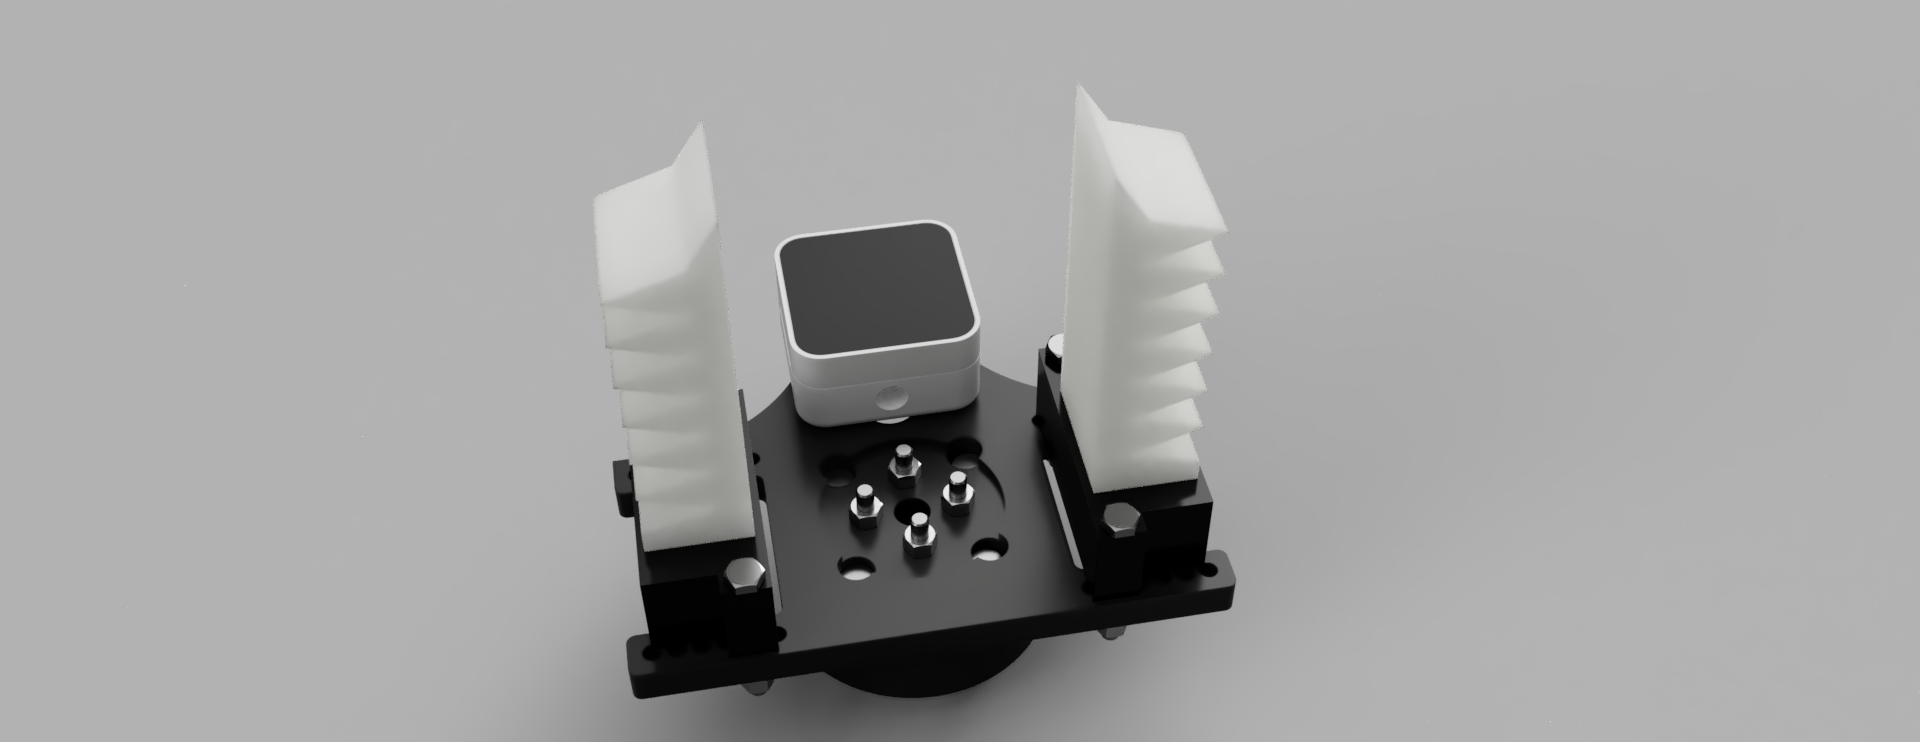
\includegraphics[width=0.7\textwidth]{figures/design/end_effector_design/ABBIRB140_EndEffector_(Assembly)_Render.png}
  \caption{End effector assembly -- render}
  \label{fig:assembly-render}
\end{figure}

\begin{figure}[ht]
  \centering
  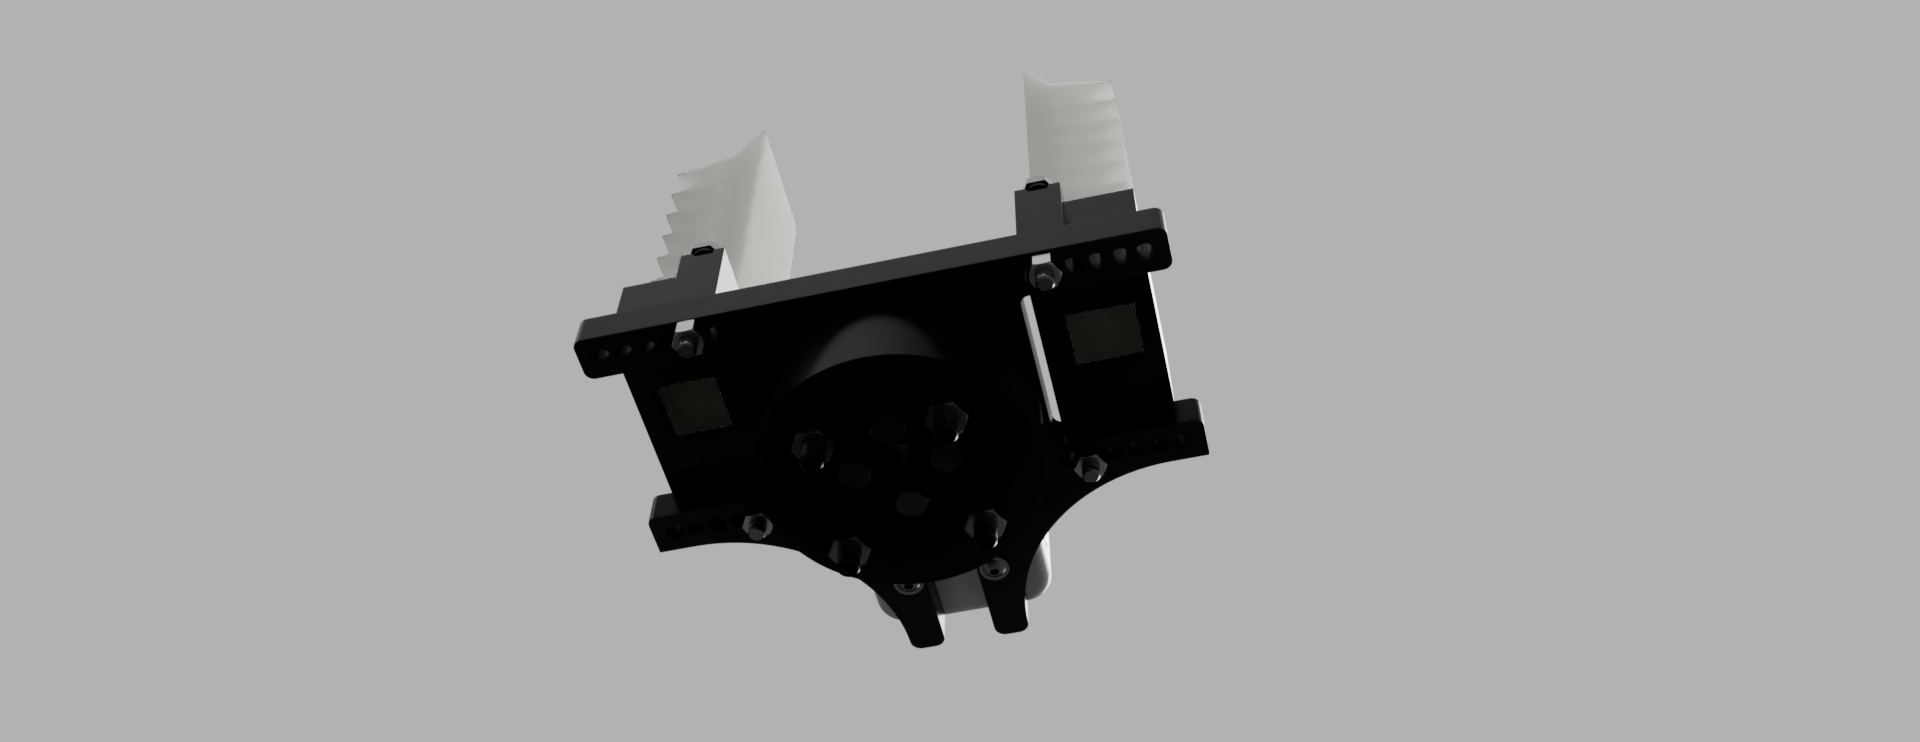
\includegraphics[width=0.7\textwidth]{figures/design/end_effector_design/ABBIRB140_EndEffector_(Assembly)_underside_render.png}
  \caption{End effector assembly -- underside render}
  \label{fig:assembly-render-underside}
\end{figure}

\subsection{Digital Twin Design}

\begin{figure}[ht]
  \centering
  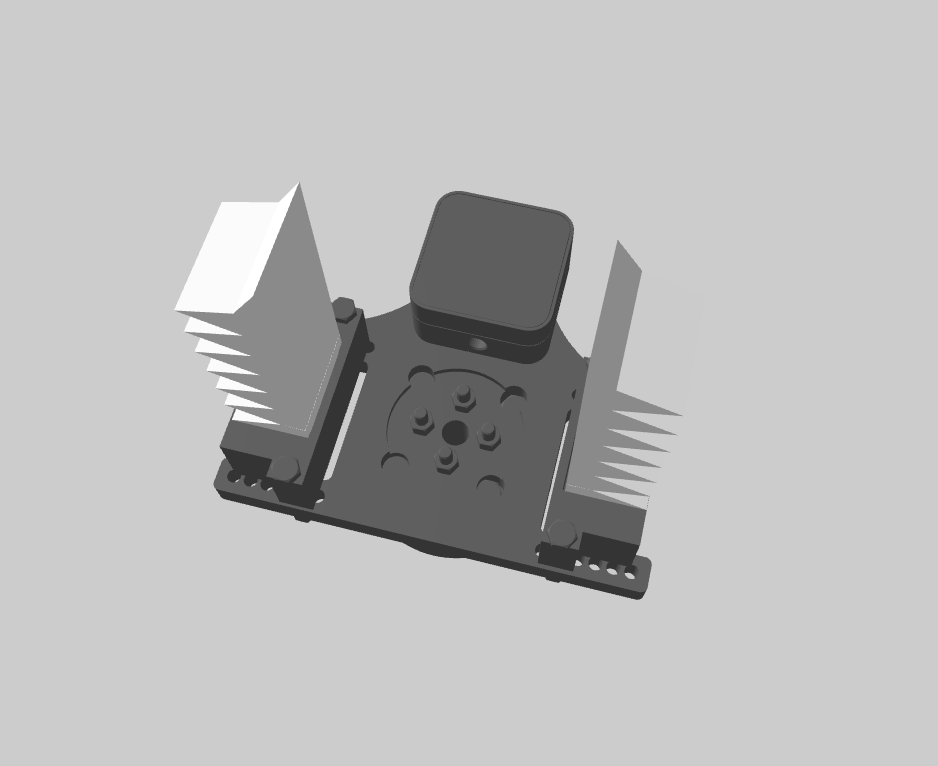
\includegraphics[width=0.7\textwidth]{figures/implementation/end_effector/end_effector_urdf_visualized.png}
  \caption{End Effector Simulation URDF Visualization gripper open}
  \label{fig:end-effector-urdf-visualization-gripper-open}
\end{figure}

\begin{figure}[ht]
  \centering
  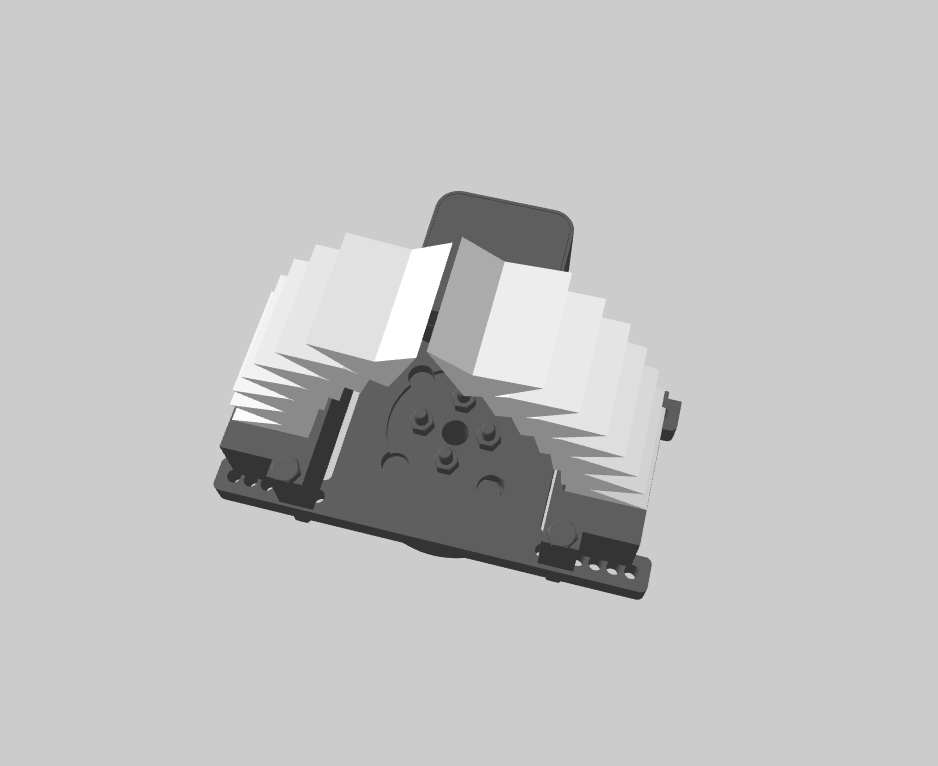
\includegraphics[width=0.7\textwidth]{figures/implementation/end_effector/end_effector_urdf_visualized_gripper_close.png}
  \caption{End Effector Simulation URDF visualization gripper closed}
  \label{fig:end-effector-urdf-visualization-gripper-closed}
\end{figure}

\begin{figure}[ht]
  \centering
  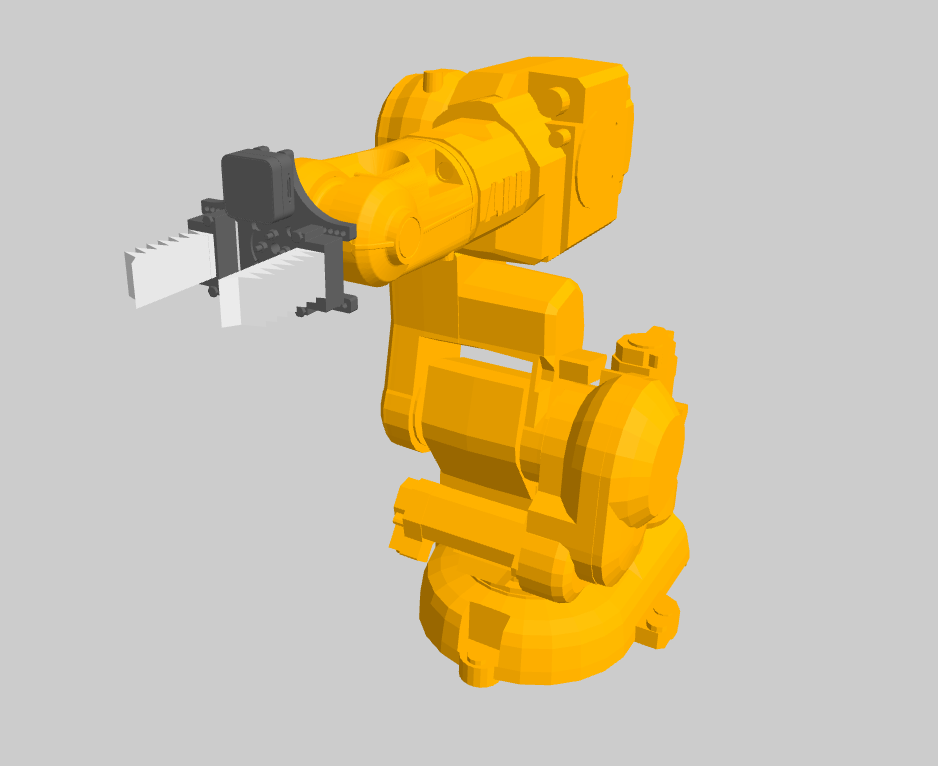
\includegraphics[width=0.7\textwidth]{figures/implementation/end_effector/irb140_urdf_visualized_with_end_effector.png}
  \caption{End Effector URDF visualization attached to IRB140 robotic URDF visualized}
  \label{fig:end-effector-urdf-visualization-attached-to-irb140}
\end{figure}


\subsection{Digital Twinning}

environment measurements

Robot Podium Design


\begin{figure}
  \centering
  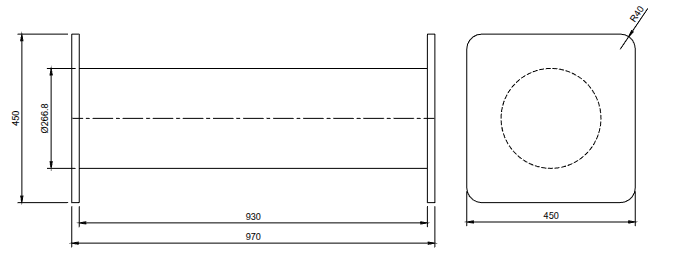
\includegraphics[width=0.7\textwidth]{./figures/design/digital  twin/robot_podium_drawing_image.png}
  \caption{Gazebo world model}
  \label{fig:world-model}  
\end{figure}


\begin{figure}
  \centering
  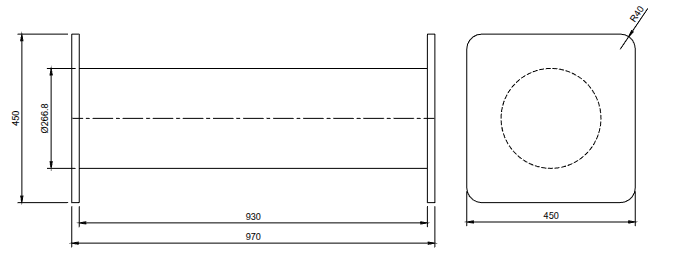
\includegraphics[width=0.7\textwidth]{./figures/design/digital  twin/robot_podium_drawing_image.png}
  \caption{Gazebo world model}
  \label{fig:world-model}  
\end{figure}

Table design

\begin{figure}
  \centering
  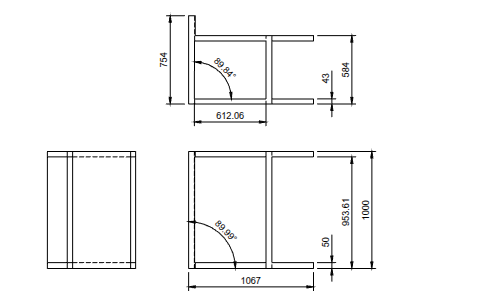
\includegraphics[width=0.7\textwidth]{./figures/design/digital  twin/table_drawing_image.png}
  \caption{Gazebo world model}
  \label{fig:world-model}  
\end{figure}

\begin{figure}
  \centering
  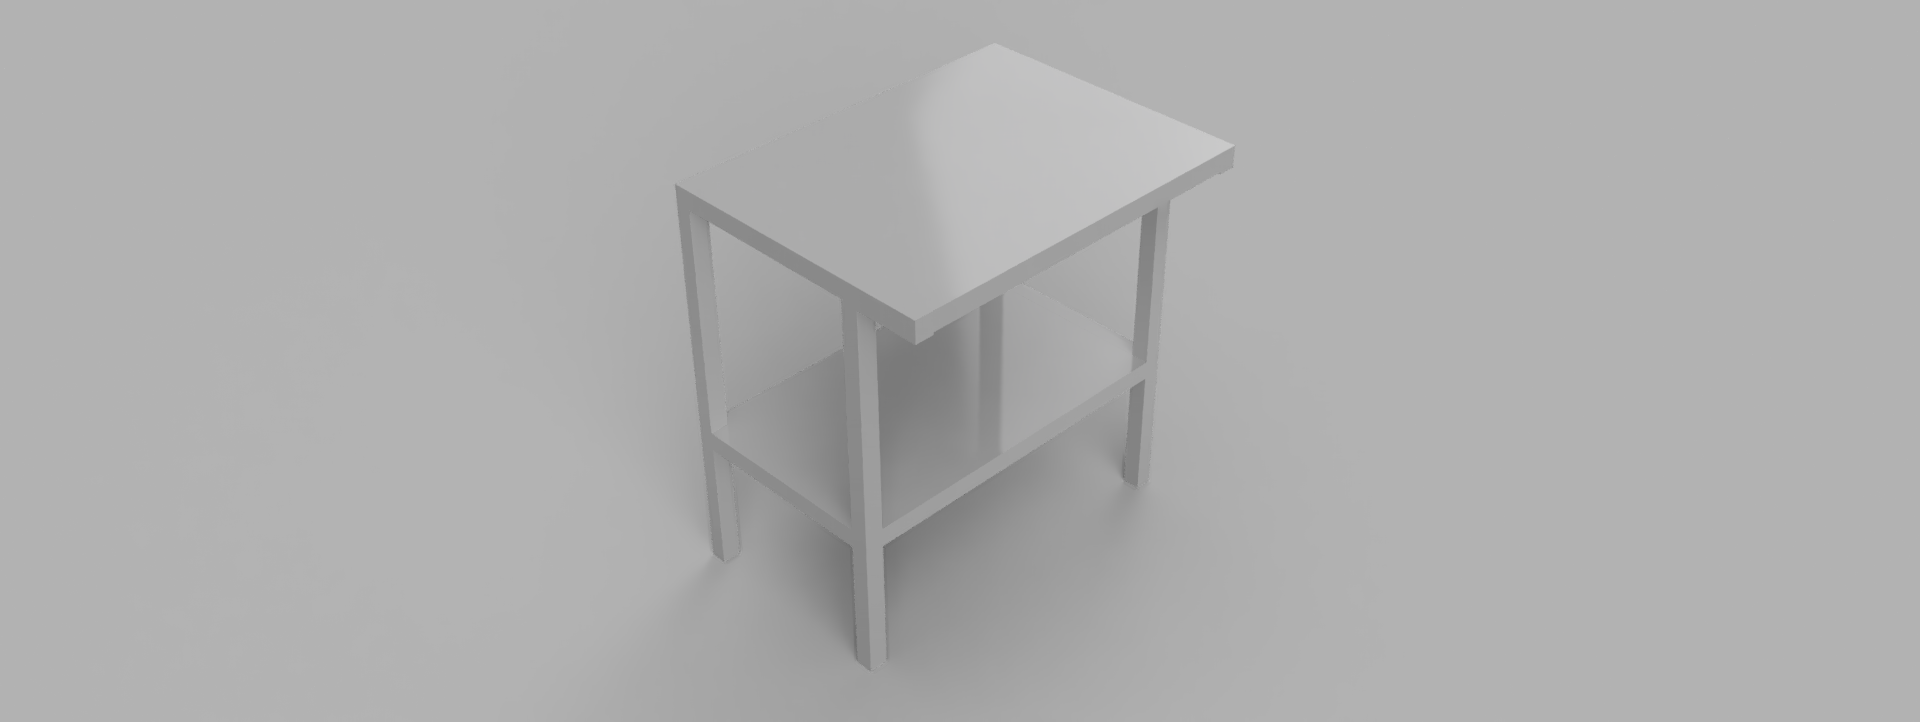
\includegraphics[width=0.7\textwidth]{./figures/design/digital  twin/Table Render.png}
  \caption{Gazebo world model}
  \label{fig:world-model}  
\end{figure}

world model

\begin{figure}
  \centering
  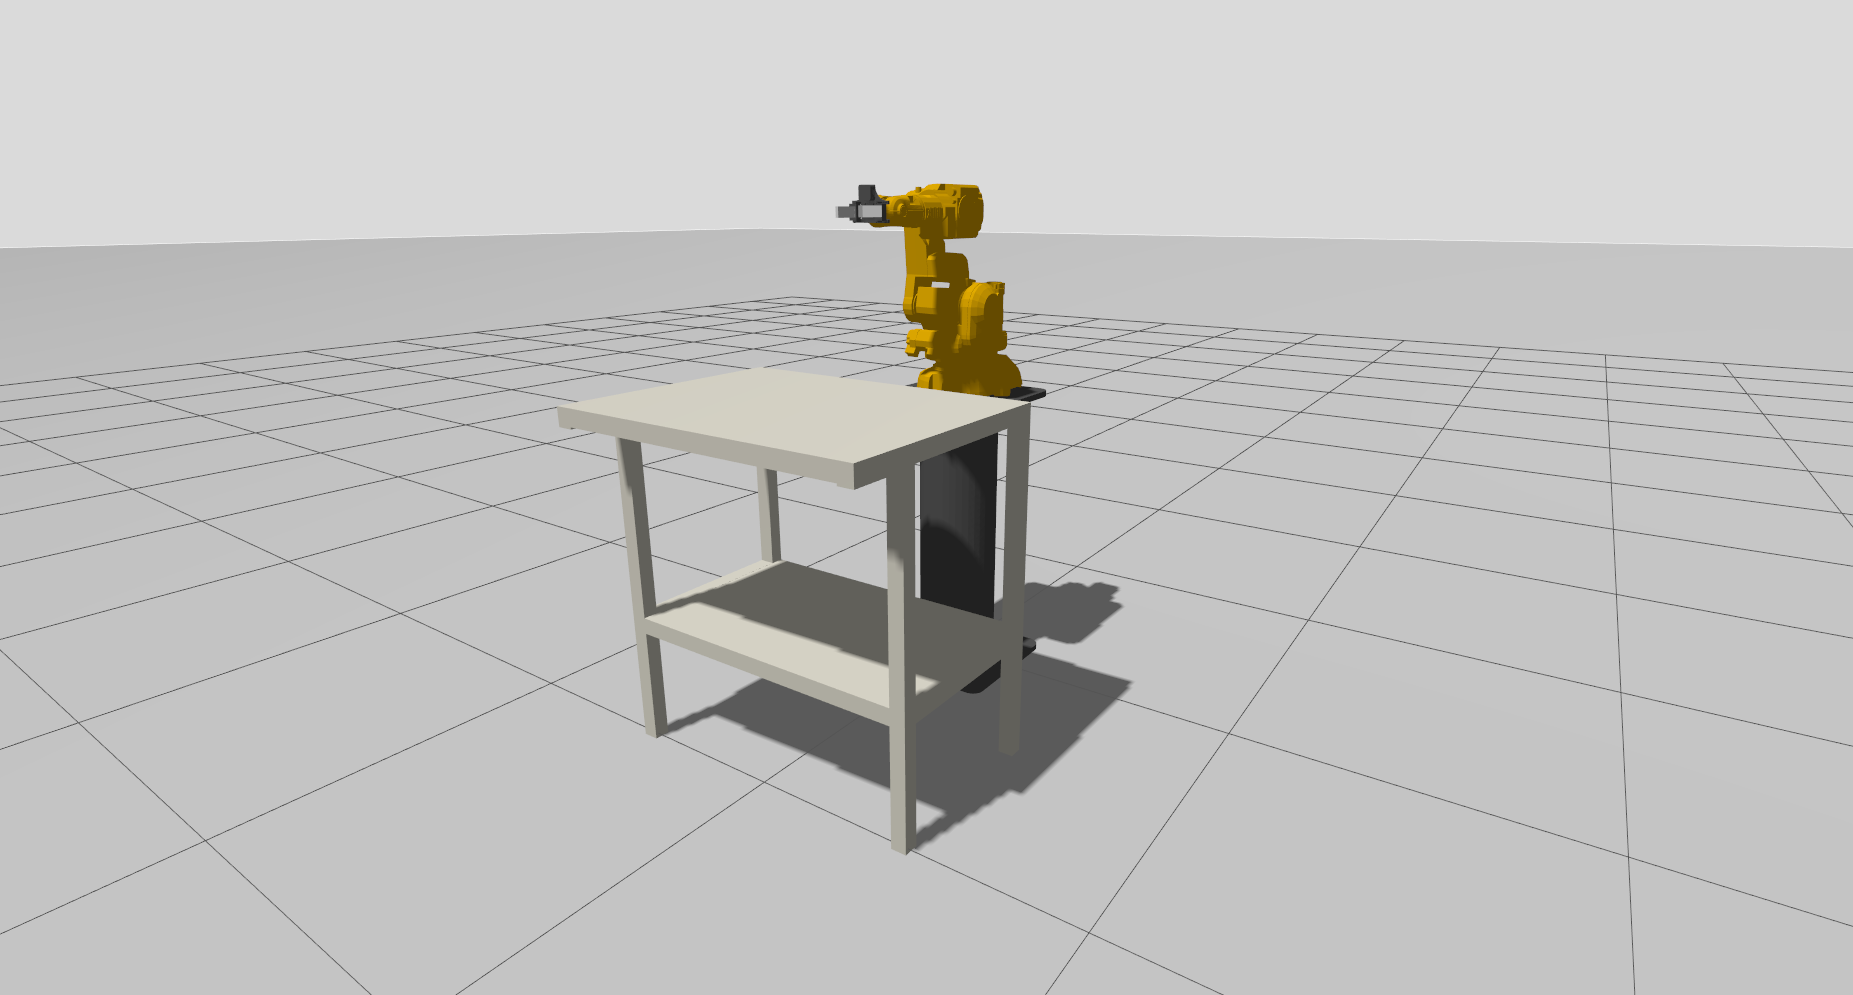
\includegraphics[width=0.7\textwidth]{./figures/implementation/world_model/world_model_1.png}
  \caption{Gazebo world model}
  \label{fig:world-model}  
\end{figure}




pneumatics design

the pneumatic flow is always the same just with different dsi for different tasks

our gripper utilizies this flow

air valve -> air resistor \(0.2MPa\)-> the solnoid valve which has this air flow FSM: TODO: ATTACH AIR FLOW FSM DIAGRAM
-> airflow resistor \(0.05MPa\) 0 -> t-splitter for the grippers -> into the silocon mould valves 

closing off the airflow for the grippers

as for electronic control for the IRC5 controller we wanted to utilize the R2.CS port on the IRB140 so that we would 
only have to plugin in a circular intake and the wiring would be3 simple, after extensive investigation into circuit charts, documentaion
and so on that was availble and even opening the robot up and tracing the wries we discovered that although utilizing multimeter and finding some of the pins on R2.CS have 
a 24v signal being drivern to them we discovered that there was no actual way to digitally drive signals by default to the pins from the IRC5 compact pendant this is due to a some hacking
needing to be done on the IRC5 to add the R2.CS as a component on the device net which it is not by default.

as for wiring XS14 port 1 and 2 for live 1 being the digital output 24v for 1 1 v for 0 for opening clsoing the grippers, 2 being opening the grippers again. and for neutral XS12 - 9.

\subsection{Components Assembly and Build}



\subsection{Issues and Future Improvements}

This is a prototype version of the end effector design, and we had some issues when actually
assembling it. These issues were twofold: first, the reference sketches I used for the finger
mounts did not give the correct distance between the mounting holes on the sides of the finger
mounts, so in future the mounting arms need to be spaced approximately 2\,mm further apart to
solve this -- we drilled through the mounting hole on the finger mount by a tiny margin to give
enough leeway to assemble it. Secondly, we did not have the M4$\times$35\,mm screws specified by
the CAD assembly, so the tool flange end effector adapter neck should in future be made shorter to
account for a 30\,mm screw length instead; to solve this problem, we ground the 50\,mm M3 screws
down by 20\,mm so we could properly mount the end effector.

One final problem was that the silicone material of the fingers did not have a high pressure
tolerance, so we had to be extremely careful with the pressure regulators connected to the
solenoid valves to ensure the fingers did not burst. This was fine, but in future it may be
useful to use a stronger material to remove this concern, as bursting a finger during testing
would have been a costly setback.

\subsection{ROS2 control}

control of the end effector is difficult. 

Simulating the robot in gazebo means utilizing two controllers, one for the robotic arm
another for the pneumatic gripper, 
the pneumatic gripper model in simulation is a combination of several different joints per 
finger, like a human finger, we can't simulate the silicone joint's for air caused closing of the finger. 


.... 

\chapter{Findings/Results and Discussion}

\subsection{Digital Twin}

\subsection{}

\chapter{Conclusions}

\chapter{Recommendations/Future Work}

\chapter{References/Bibliography}

\begin{itemize}
  \item \url{https://www.kaggle.com/datasets/ronanpickell/b100-lego-detection-dataset?resource=download} -- YOLO LEGO detection training dataset
\end{itemize}

\appendix

\chapter{URDF / Xacro Source}
\label{app:urdf}

The robot and end-effector model is defined as a set of URDF/Xacro files. The
three listings below are given in include order: the top-level robot description
(\texttt{abb\_irb140.urdf.xacro}), followed by the two macros it pulls in for the
pneumatic gripper body (\texttt{irb140\_pneumonic\_gripper.xacro}) and its
compliant fingers (\texttt{irb140\_pneumonic\_gripper\_finger.xacro}).

\section{Top-level robot description}

\begin{lstlisting}[language=XML,caption={Top-level robot description; instantiates the ABB IRB140 links/joints and includes the pneumatic gripper macro.},label={lst:urdf-robot}]
<?xml version="1.0" ?>

<robot xmlns:xacro="https://www.ros.org/wiki/xacro" name="abb_irb140"> 

  <xacro:include filename="$(find abb_irb140_description)/urdf/irb140_pneumonic_gripper.xacro"/>

  <material name="abb_orange">
    <color rgba="1 0.43 0 1"/>
  </material>
  <material name="yellow">
    <color rgba="0 1 1 1"/>
  </material>
  <link name="world"/>
  <joint name="world-base_link" type="fixed">
    <origin rpy="0 0 0" xyz="0 0 0"/>
    <parent link="world"/>
    <child link="base_link"/>
  </joint>
  <link name="base_link">
    <visual>
      <origin rpy="0 0 0" xyz="0 0 0"/>
      <geometry>
        <mesh filename="package://abb_irb140_description/meshes/abb_irb140/visual/base_link.stl" scale="0.208333 0.208333 0.208333"/>
      </geometry>
      <material name="abb_orange"/>
    </visual>
    <collision>
      <geometry>
        <mesh filename="package://abb_irb140_description/meshes/abb_irb140/collision/base_link.stl" scale="0.208333 0.208333 0.208333"/>
      </geometry>
    </collision>
    <!-- mass/inertia computed from the visual mesh geometry (tetrahedron
         decomposition, uniform density scaled so the 7 links sum to the
         published IRB140 mass of ~98 kg); see scratchpad/compute_inertials.py -->
    <inertial>
      <origin xyz="-0.067289 0.00033 0.049151" rpy="0 0 0"/>
      <mass value="26.383023"/>
      <inertia ixx="0.149473" ixy="-0.000014" ixz="0.010503" iyy="0.239263" iyz="0.001206" izz="0.352558"/>
    </inertial>
  </link>
  <link name="link_1">
    <visual>
      <origin rpy="0 0 0" xyz="0 0 0"/>
      <geometry>
        <mesh filename="package://abb_irb140_description/meshes/abb_irb140/visual/link_1.stl" scale="0.208333 0.208333 0.208333"/>
      </geometry>
      <material name="abb_orange"/>
    </visual>
    <collision>
      <origin rpy="0 0 0" xyz="0 0 0"/>
      <geometry>
        <mesh filename="package://abb_irb140_description/meshes/abb_irb140/collision/link_1.stl" scale="0.208333 0.208333 0.208333"/>
      </geometry>
    </collision>
    <inertial>
      <origin xyz="0.023053 0.035938 0.216046" rpy="0 0 0"/>
      <mass value="34.629380"/>
      <inertia ixx="0.342938" ixy="-0.000999" ixz="-0.035343" iyy="0.310928" iyz="-0.046431" izz="0.30792"/>
    </inertial>
  </link>
  <link name="link_2">
    <visual>
      <origin rpy="0 0 0" xyz="-0.058333 0 -0.2875"/>
      <geometry>
        <mesh filename="package://abb_irb140_description/meshes/abb_irb140/visual/link_2.stl" scale="0.208333 0.208333 0.208333"/>
      </geometry>
      <material name="abb_orange"/>
    </visual>
    <collision>
      <origin rpy="0 0 0" xyz="-0.058333 0 -0.2875"/>
      <geometry>
        <mesh filename="package://abb_irb140_description/meshes/abb_irb140/collision/link_2.stl" scale="0.208333 0.208333 0.208333"/>
      </geometry>
    </collision>
    <inertial>
      <origin xyz="-0.008898 -0.075815 0.163852" rpy="0 0 0"/>
      <mass value="16.116764"/>
      <inertia ixx="0.222755" ixy="0.000738" ixz="-0.002616" iyy="0.188088" iyz="0.025713" izz="0.064275"/>
    </inertial>
  </link>
  <link name="link_3">
    <visual>
      <origin rpy="0 0 0" xyz="-0.058333 0 -0.583333"/>
      <geometry>
        <mesh filename="package://abb_irb140_description/meshes/abb_irb140/visual/link_3.stl" scale="0.208333 0.208333 0.208333"/>
      </geometry>
      <material name="abb_orange"/>
    </visual>
    <collision>
      <origin rpy="0 0 0" xyz="-0.058333 0 -0.583333"/>
      <geometry>
        <mesh filename="package://abb_irb140_description/meshes/abb_irb140/collision/link_3.stl" scale="0.208333 0.208333 0.208333"/>
      </geometry>
    </collision>
    <inertial>
      <origin xyz="0.014339 0.006218 -0.004026" rpy="0 0 0"/>
      <mass value="16.752833"/>
      <inertia ixx="0.045722" ixy="0.00413" ixz="0.002649" iyy="0.12903" iyz="0.00052" izz="0.117339"/>
    </inertial>
  </link>
  <link name="link_4">
    <visual>
      <origin rpy="0 0 0" xyz="-0.058333 0 -0.583333"/>
      <geometry>
        <mesh filename="package://abb_irb140_description/meshes/abb_irb140/visual/link_4.stl" scale="0.208333 0.208333 0.208333"/>
      </geometry>
      <material name="abb_orange"/>
    </visual>
    <collision>
      <origin rpy="0 0 0" xyz="-0.058333 0 -0.583333"/>
      <geometry>
        <mesh filename="package://abb_irb140_description/meshes/abb_irb140/collision/link_4.stl" scale="0.208333 0.208333 0.208333"/>
      </geometry>
    </collision>
    <inertial>
      <origin xyz="0.25463 -0.001001 -0.000524" rpy="0 0 0"/>
      <mass value="3.755635"/>
      <inertia ixx="0.004931" ixy="0.000293" ixz="-0.000085" iyy="0.01037" iyz="0.000005" izz="0.011621"/>
    </inertial>
  </link>
  <link name="link_5">
    <visual>
      <origin rpy="0 0 0" xyz="-0.36875 0 -0.583333"/>
      <geometry>
        <mesh filename="package://abb_irb140_description/meshes/abb_irb140/visual/link_5.stl" scale="0.208333 0.208333 0.208333"/>
      </geometry>
      <material name="abb_orange"/>
    </visual>
    <collision>
      <origin rpy="0 0 0" xyz="-0.36875 0 -0.583333"/>
      <geometry>
        <mesh filename="package://abb_irb140_description/meshes/abb_irb140/collision/link_5.stl" scale="0.208333 0.208333 0.208333"/>
      </geometry>
    </collision>
    <inertial>
      <origin xyz="-0.000809 0.000507 0.000589" rpy="0 0 0"/>
      <mass value="0.307952"/>
      <inertia ixx="0.000101" ixy="0" ixz="0" iyy="0.000159" iyz="0" izz="0.000098"/>
    </inertial>
  </link>
  <link name="link_6">
    <visual>
      <origin rpy="0 0 0" xyz="-0.36875 0 -0.583333"/>
      <geometry>
        <mesh filename="package://abb_irb140_description/meshes/abb_irb140/visual/link_6.stl" scale="0.208333 0.208333 0.208333"/>
      </geometry>
      <material name="abb_orange"/>
    </visual>
    <collision>
      <origin rpy="0 0 0" xyz="-0.36875 0 -0.583333"/>
      <geometry>
        <mesh filename="package://abb_irb140_description/meshes/abb_irb140/collision/link_6.stl" scale="0.208333 0.208333 0.208333"/>
      </geometry>
    </collision>
    <inertial>
      <origin xyz="0.043159 0.000003 0.000479" rpy="0 0 0"/>
      <mass value="0.054413"/>
      <inertia ixx="0.000008" ixy="0" ixz="0" iyy="0.000009" iyz="0" izz="0.000009"/>
    </inertial>
  </link>
  <link name="tool0"/>
  <joint name="joint_1" type="revolute">
    <origin rpy="0 0 0" xyz="0 0 0"/>
    <parent link="base_link"/>
    <child link="link_1"/>
    <axis xyz="0 0 1"/>
    <limit effort="200" lower="-3.1416" upper="3.1416" velocity="2.618"/>
  </joint>
  <joint name="joint_2" type="revolute">
    <origin rpy="0 0 0" xyz="0.058333 0 0.2875"/>
    <parent link="link_1"/>
    <child link="link_2"/>
    <axis xyz="0 1 0"/>
    <limit effort="200" lower="-1.7453" upper="1.9199" velocity="2.618"/>
  </joint>
  <joint name="joint_3" type="revolute">
    <origin rpy="0 0 0" xyz="0 0 0.295833"/>
    <parent link="link_2"/>
    <child link="link_3"/>
    <axis xyz="0 1 0"/>
    <limit effort="150" lower="-1.0472" upper="1.1345" velocity="2.618"/>
  </joint>
  <joint name="joint_4" type="revolute">
    <origin rpy="0 0 0" xyz="0 0 0"/>
    <parent link="link_3"/>
    <child link="link_4"/>
    <axis xyz="1 0 0"/>
    <limit effort="50" lower="-3.49" upper="3.49" velocity="6.2832"/>
  </joint>
  <joint name="joint_5" type="revolute">
    <origin rpy="0 0 0" xyz="0.310417 0 0"/>
    <parent link="link_4"/>
    <child link="link_5"/>
    <axis xyz="0 1 0"/>
    <limit effort="50" lower="-2.0944" upper="2.0944" velocity="6.2832"/>
  </joint>
  <joint name="joint_6" type="revolute">
    <origin rpy="0 0 0" xyz="0 0 0.004167"/>
    <parent link="link_5"/>
    <child link="link_6"/>
    <axis xyz="1 0 0"/>
    <limit effort="20" lower="-6.9813" upper="6.9813" velocity="7.854"/>
  </joint>
  <joint name="joint_6-tool0" type="fixed">
    <parent link="link_6"/>
    <child link="tool0"/>
    <origin rpy="0 1.57079632679 0" xyz="0 0 0"/>
  </joint>
  <link name="base"/>
  <joint name="base_link-base" type="fixed">
    <origin rpy="0 0 0" xyz="0 0 0"/>
    <parent link="base_link"/>
    <child link="base"/>
  </joint>

  <xacro:pneumatic_gripper name="pneumatic_gripper" parent="tool0" xyz="0.00 0.0 0.08" rpy="0 0 3.142"/>

  <!-- =================================================================== -->
  <!-- ros2_control + Gazebo Sim                                           -->
  <!-- =================================================================== -->

  <!-- ros2_control hardware for the 6 arm joints. gz_ros2_control's
       GazeboSimSystem reads/writes these interfaces straight from the gz-sim
       physics engine. command/state interfaces match config/controllers.yaml
       (arm_controller: position command; position + velocity state). -->
  <ros2_control name="GazeboSimSystem" type="system">
    <hardware>
      <plugin>gz_ros2_control/GazeboSimSystem</plugin>
    </hardware>
    <joint name="joint_1">
      <command_interface name="position">
        <param name="min">-3.1416</param>
        <param name="max">3.1416</param>
      </command_interface>
      <state_interface name="position"/>
      <state_interface name="velocity"/>
    </joint>
    <joint name="joint_2">
      <command_interface name="position">
        <param name="min">-1.7453</param>
        <param name="max">1.9199</param>
      </command_interface>
      <state_interface name="position"/>
      <state_interface name="velocity"/>
    </joint>
    <joint name="joint_3">
      <command_interface name="position">
        <param name="min">-1.0472</param>
        <param name="max">1.1345</param>
      </command_interface>
      <state_interface name="position"/>
      <state_interface name="velocity"/>
    </joint>
    <joint name="joint_4">
      <command_interface name="position">
        <param name="min">-3.49</param>
        <param name="max">3.49</param>
      </command_interface>
      <state_interface name="position"/>
      <state_interface name="velocity"/>
    </joint>
    <joint name="joint_5">
      <command_interface name="position">
        <param name="min">-2.0944</param>
        <param name="max">2.0944</param>
      </command_interface>
      <state_interface name="position"/>
      <state_interface name="velocity"/>
    </joint>
    <joint name="joint_6">
      <command_interface name="position">
        <param name="min">-6.9813</param>
        <param name="max">6.9813</param>
      </command_interface>
      <state_interface name="position"/>
      <state_interface name="velocity"/>
    </joint>

    <!-- Pneumatic gripper. Only the left finger's first joint is a real
         driver (position command interface); the other 11 finger joints are
         declared mimic="true" here and carry <mimic> elements in
         irb140_pneumonic_gripper_finger.xacro, so a single
         GripperActionController (config/controllers.yaml: gripper_controller)
         opens/closes both fingers. Mimic joints may only export state
         interfaces. -->
    <joint name="pneumatic_gripper_left_link_1_to_link_2">
      <!-- Software travel limit for the driver joint: -0.0698 ("closed") is
           deliberately kept 0.02 rad inside the -0.09 mechanical joint limit
           (see irb140_pneumonic_gripper_finger.xacro) so a closed gripper is
           resting, not pegged on the hard stop; opening from closed is then
           a free move the weak position gain can complete without stalling. -->
      <command_interface name="position">
        <param name="min">-0.0698</param>
        <param name="max">0.0</param>
      </command_interface>
      <state_interface name="position"/>
      <state_interface name="velocity"/>
    </joint>
    <joint name="pneumatic_gripper_left_link_2_to_link_3" mimic="true">
      <state_interface name="position"/>
      <state_interface name="velocity"/>
    </joint>
    <joint name="pneumatic_gripper_left_link_3_to_link_4" mimic="true">
      <state_interface name="position"/>
      <state_interface name="velocity"/>
    </joint>
    <joint name="pneumatic_gripper_left_link_4_to_link_5" mimic="true">
      <state_interface name="position"/>
      <state_interface name="velocity"/>
    </joint>
    <joint name="pneumatic_gripper_left_link_5_to_link_6" mimic="true">
      <state_interface name="position"/>
      <state_interface name="velocity"/>
    </joint>
    <joint name="pneumatic_gripper_left_link_6_to_link_7" mimic="true">
      <state_interface name="position"/>
      <state_interface name="velocity"/>
    </joint>
    <joint name="pneumatic_gripper_right_link_1_to_link_2" mimic="true">
      <state_interface name="position"/>
      <state_interface name="velocity"/>
    </joint>
    <joint name="pneumatic_gripper_right_link_2_to_link_3" mimic="true">
      <state_interface name="position"/>
      <state_interface name="velocity"/>
    </joint>
    <joint name="pneumatic_gripper_right_link_3_to_link_4" mimic="true">
      <state_interface name="position"/>
      <state_interface name="velocity"/>
    </joint>
    <joint name="pneumatic_gripper_right_link_4_to_link_5" mimic="true">
      <state_interface name="position"/>
      <state_interface name="velocity"/>
    </joint>
    <joint name="pneumatic_gripper_right_link_5_to_link_6" mimic="true">
      <state_interface name="position"/>
      <state_interface name="velocity"/>
    </joint>
    <joint name="pneumatic_gripper_right_link_6_to_link_7" mimic="true">
      <state_interface name="position"/>
      <state_interface name="velocity"/>
    </joint>
  </ros2_control>

  <!-- Brings up a controller_manager inside gz-sim once the entity is spawned.
       CONTROLLERS_YAML_PATH is a literal token that launch/gazebo.launch.py
       rewrites to the installed config/controllers.yaml path before the URDF
       is published (gz_ros2_control does not evaluate $(find pkg) itself when
       the description is passed through as plain text). -->
  <gazebo>
    <plugin filename="gz_ros2_control-system"
            name="gz_ros2_control::GazeboSimROS2ControlPlugin">
      <parameters>CONTROLLERS_YAML_PATH</parameters>
    </plugin>
  </gazebo>
</robot>


\end{lstlisting}

\section{Pneumatic gripper body macro}

\begin{lstlisting}[language=XML,caption={Pneumatic gripper body macro: 3D-printed housing, flange mount, optional wrist RGBD camera and \texttt{ros2\_control} hooks.},label={lst:urdf-gripper}]
<?xml version="1.0" encoding="UTF-8"?>
<robot xmlns:xacro="http://www.ros.org/wiki/xacro" name="pneumatic_gripper">

<xacro:include filename="$(find abb_irb140_description)/urdf/irb140_pneumonic_gripper_finger.xacro"/>

<!-- Set include_camera:=false at xacro time to drop the wrist RGBD camera. -->
<xacro:arg name="include_camera" default="true"/>

<!-- 3D-printed PLA housing: solid PLA is ~1240 kg/m^3; with typical printed
     wall/infill this shell is roughly half that, so ~650 kg/m^3 over the
     bounding box gives a realistic ~0.45 kg body. -->
<xacro:property name="pla_density" value="650.0"/>

<xacro:macro name="pneumatic_gripper" params="name parent xyz:='0 0 0' rpy:='0 0 0'">

    <!-- Attach the gripper body to the robot flange.
         xyz/rpy are expressed in the parent (tool0) frame; set xyz to
         shift the gripper along the flange axes. -->
    <joint name="${name}_to_${parent}" type="fixed">
        <parent link="${parent}"/>
        <child link="${name}_base_link"/>
        <origin xyz="${xyz}" rpy="${rpy}"/>
    </joint>

    <link name="${name}_base_link">
        <visual>
            <origin xyz="0 0 -0.03105" rpy="0 0 0"/>
            <geometry>
                <mesh filename="package://abb_irb140_description/meshes/abb_irb140_pneumonic_end_effector/visual/ABBIRB140_EndEffector.stl" scale="0.001 0.001 0.001"/>
            </geometry>
            <material name="plastic">
                <color rgba="0.11 0.11 0.11 1"/>
            </material>
        </visual>

        <collision>
            <origin xyz="0.0165 0 -0.005" rpy="0 0 0"/>
            <geometry>
                <box size="0.1 0.125 0.062"/>
            </geometry>
        </collision>

        <xacro:solid_box_inertial sx="0.1" sy="0.125" sz="0.062" density="${pla_density}">
            <origin xyz="0.0165 0 -0.005" rpy="0 0 0"/>
        </xacro:solid_box_inertial>
    </link>

    <!-- Spawn left and right gripper fingers.
         The offset/rotation for each finger is passed straight into the
         finger macro's base joint (its <origin> block).
         The left finger's first joint (${name}_left_link_1_to_link_2) is the
         single driver: it gets the ros2_control position command interface in
         irb140.xacro, and the other 11 finger joints mimic it, so one
         GripperActionController opens/closes both fingers. -->
    <xacro:pneumatic_gripper_finger name="${name}_left" parent="${name}_base_link">
        <origin xyz="0.0 0.046 0.0071" rpy="0.0 0.0 1.57"/>
    </xacro:pneumatic_gripper_finger>

    <xacro:pneumatic_gripper_finger name="${name}_right" parent="${name}_base_link"
                                    mimic_master="${name}_left_link_1_to_link_2">
        <origin xyz="-0.008 -0.046 0.0071" rpy="0.0 0.0 -1.57"/>
    </xacro:pneumatic_gripper_finger>

    <!-- ================================================================= -->
    <!-- Eye-in-hand RGBD camera                                           -->
    <!-- ================================================================= -->
    <!-- Link/sensor/topic names are deliberately un-namespaced
         (depth_camera / rgbd_camera): config/rgbd_bridge.yaml and
         launch/gazebo.launch.py refer to them by those fixed names. Only one
         gripper is ever instantiated, so there is no collision. -->
    <xacro:if value="$(arg include_camera)">

        <!-- Geometry-less sensor frame: the physical camera is already
             sculpted into the base_link visual mesh, so this link carries no
             visual/collision of its own (that would just duplicate the mesh
             as a second, floating box). It exists purely so the Gazebo
             rgbd_camera sensor below has a link to attach to, positioned and
             rotated (local +X is the gz camera view axis) to coincide with
             the real camera on the mesh, along the gripper's approach
             direction (+Z of ${name}_base_link). Tune the joint origin below
             to reframe the grasp view. -->
        <link name="depth_camera">
            <inertial>
                <mass value="0.05"/>
                <inertia ixx="1e-5" ixy="0" ixz="0" iyy="1e-5" iyz="0" izz="1e-5"/>
            </inertial>
        </link>

        <joint name="${name}_to_depth_camera" type="fixed">
            <parent link="${name}_base_link"/>
            <child link="depth_camera"/>
            <origin xyz="-0.025 0.0 0.3" rpy="3.14159265359 0 0"/>
        </joint>

        <!-- Keep depth_camera as its own link/frame in the converted SDF
             instead of letting urdf2sdf lump it (and the sensor) back into
             link_6 through the fixed-joint chain. -->
        <gazebo reference="${name}_to_depth_camera">
            <preserveFixedJoint>true</preserveFixedJoint>
            <disableFixedJointLumping>true</disableFixedJointLumping>
        </gazebo>

        <!-- Standard ROS optical frame (z forward, x right, y down) relative to
             the camera body link; camera_info / point clouds are published in
             this frame. -->
        <link name="depth_camera_optical"/>
        <joint name="depth_camera_to_optical" type="fixed">
            <parent link="depth_camera"/>
            <child link="depth_camera_optical"/>
            <origin xyz="0 0 0" rpy="0 -1.57 0"/>
        </joint>

        <!-- reference="depth_camera" binds the gz-sim sensor to that link.
             worlds/robot_lab.world already loads gz-sim-sensors-system. gz
             publishes /rgbd_camera/{image,depth_image,points,camera_info};
             those are remapped to RealSense-style ROS 2 names by
             config/rgbd_bridge.yaml in launch/gazebo.launch.py. -->
        <gazebo reference="depth_camera">
            <sensor name="rgbd_camera" type="rgbd_camera">
                <always_on>1</always_on>
                <update_rate>30</update_rate>
                <visualize>true</visualize>
                <topic>rgbd_camera</topic>
                <gz_frame_id>depth_camera</gz_frame_id>
                <camera>
                    <horizontal_fov>1.3962634</horizontal_fov>
                    <image>
                        <width>640</width>
                        <height>480</height>
                        <format>R8G8B8</format>
                    </image>
                    <clip>
                        <near>0.1</near>
                        <far>15</far>
                    </clip>
                    <depth_camera>
                        <clip>
                            <near>0.1</near>
                            <far>15</far>
                        </clip>
                    </depth_camera>
                    <optical_frame_id>depth_camera_optical</optical_frame_id>
                </camera>
            </sensor>
        </gazebo>

    </xacro:if>

</xacro:macro>

</robot>
\end{lstlisting}

\section{Compliant gripper finger macro}

\begin{lstlisting}[language=XML,caption={Compliant multi-segment gripper finger macro: mimic joints and cast-silicone inertial estimates.},label={lst:urdf-finger}]
<?xml version="1.0" encoding="UTF-8"?>
<robot xmlns:xacro="http://www.ros.org/wiki/xacro" name="pneumatic_gripper_finger">
    
    <!-- Properties -->
    <xacro:property name="mesh_scale" value="0.001 0.001 0.001"/>
    <xacro:property name="collision_scale" value="0.025 0.03 0.1"/>
    <!-- Mechanical hard stop for each finger segment. The GripperActionController
         is commanded to -0.0698 for "closed" (command_interface min in
         irb140.xacro), so this limit sits 0.02 rad beyond that: a closed gripper
         rests short of the stop instead of jamming against it, which is what let
         a single-shot open stall out from the fully-closed pose. -->
    <xacro:property name="joint_lower_limit" value="-0.09"/>

    <!-- Cast silicone rubber (Dragon Skin / Ecoflex class), ~1100 kg/m^3.
         Raise this if the finger chain jitters in Gazebo; it scales every
         segment mass and inertia together. -->
    <xacro:property name="silicone_density" value="1100.0"/>

    <material name="offwhite">
        <color rgba="0.8 0.8 0.8 1"/>
    </material>

    <!-- Solid-box mass + inertia from full box dimensions (sx,sy,sz) and a
         material density. Inertia is taken about the box centre, so pass the
         same *origin used for the matching <collision> box. -->
    <xacro:macro name="solid_box_inertial" params="sx sy sz density *origin">
        <inertial>
            <xacro:insert_block name="origin"/>
            <mass value="${density * sx * sy * sz}"/>
            <inertia ixx="${density * sx * sy * sz * (sy*sy + sz*sz) / 12.0}" ixy="0.0" ixz="0.0"
                     iyy="${density * sx * sy * sz * (sx*sx + sz*sz) / 12.0}" iyz="0.0"
                     izz="${density * sx * sy * sz * (sx*sx + sy*sy) / 12.0}"/>
        </inertial>
    </xacro:macro>

    <!-- Macro for the finger assembly.
         mimic_master: leave empty on the driver finger, so its own
         ${name}_link_1_to_link_2 becomes the joint everything else mimics.
         Set it to that joint's name on the second finger so both fingers
         follow a single ros2_control command interface. -->
    <xacro:macro name="pneumatic_gripper_finger" params="name parent mimic_master:='' *origin">

        <!-- Joint that every non-driver segment of this finger mimics.
             mimic_master is empty on the driver finger, so it defaults to
             mimicking its own ${name}_link_1_to_link_2 joint; the other
             finger passes in the driver's joint name to override that.
             Written with xacro:unless (rather than a python
             "X if Y else Z" property expression) so this still parses under
             JS-based xacro tools (e.g. IDE xacro/URDF previews), not just
             the Python xacro used at colcon-build time. -->
        <xacro:property name="_master" value="${name}_link_1_to_link_2"/>
        <xacro:unless value="${mimic_master == ''}">
            <xacro:property name="_master" value="${mimic_master}"/>
        </xacro:unless>

        <link name="${name}_link_1">
            <visual>
                <geometry>
                    <mesh filename="package://abb_irb140_description/meshes/abb_irb140_pneumonic_end_effector/visual/finger_visual/visual/link_1.stl" scale="${mesh_scale}"/>
                </geometry>
                <material name="offwhite"/>
            </visual>
            <collision>
                <origin xyz="0 0.005 0.009" rpy="0 0 0"/>
                <geometry>
                    <box size="0.025 0.03 0.022"/>
                </geometry>
            </collision>
            <xacro:solid_box_inertial sx="0.025" sy="0.03" sz="0.022" density="${silicone_density}">
                <origin xyz="0 0.005 0.009" rpy="0 0 0"/>
            </xacro:solid_box_inertial>
        </link>

        <link name="${name}_link_2">
            <visual>
                <geometry>
                    <mesh filename="package://abb_irb140_description/meshes/abb_irb140_pneumonic_end_effector/visual/finger_visual/visual/link_2.stl" scale="${mesh_scale}"/>
                </geometry>
                <material name="offwhite"/>
            </visual>
            <collision>
                <origin xyz="0 0 0.025" rpy="0 0 0"/>
                <geometry>
                    <box size="0.025 0.03 0.011"/>
                </geometry>
            </collision>
            <xacro:solid_box_inertial sx="0.025" sy="0.03" sz="0.011" density="${silicone_density}">
                <origin xyz="0 0 0.025" rpy="0 0 0"/>
            </xacro:solid_box_inertial>
        </link>

        <link name="${name}_link_3">
            <visual>
                <geometry>
                    <mesh filename="package://abb_irb140_description/meshes/abb_irb140_pneumonic_end_effector/visual/finger_visual/visual/link_3.stl" scale="${mesh_scale}"/>
                </geometry>
                <material name="offwhite"/>
            </visual>
            <collision>
                <origin xyz="0 0 0.035" rpy="0 0 0"/>
                <geometry>
                    <box size="0.025 0.03 0.011"/>
                </geometry>
            </collision>
            <xacro:solid_box_inertial sx="0.025" sy="0.03" sz="0.011" density="${silicone_density}">
                <origin xyz="0 0 0.035" rpy="0 0 0"/>
            </xacro:solid_box_inertial>
        </link>

        <link name="${name}_link_4">
            <visual>
                <geometry>
                    <mesh filename="package://abb_irb140_description/meshes/abb_irb140_pneumonic_end_effector/visual/finger_visual/visual/link_4.stl" scale="${mesh_scale}"/>
                </geometry>
                <material name="offwhite"/>
            </visual>
            <collision>
                <origin xyz="0 0 0.055" rpy="0 0 0"/>
                <geometry>
                    <box size="0.025 0.03 0.011"/>
                </geometry>
            </collision>
            <xacro:solid_box_inertial sx="0.025" sy="0.03" sz="0.011" density="${silicone_density}">
                <origin xyz="0 0 0.055" rpy="0 0 0"/>
            </xacro:solid_box_inertial>
        </link>

        <link name="${name}_link_5">
            <visual>
                <geometry>
                    <mesh filename="package://abb_irb140_description/meshes/abb_irb140_pneumonic_end_effector/visual/finger_visual/visual/link_5.stl" scale="${mesh_scale}"/>
                </geometry>
                <material name="offwhite"/>
            </visual>
            <collision>
                <origin xyz="0 0 0.065" rpy="0 0 0"/>
                <geometry>
                    <box size="0.025 0.03 0.011"/>
                </geometry>
            </collision>
            <xacro:solid_box_inertial sx="0.025" sy="0.03" sz="0.011" density="${silicone_density}">
                <origin xyz="0 0 0.065" rpy="0 0 0"/>
            </xacro:solid_box_inertial>
        </link>

        <link name="${name}_link_6">
            <visual>
                <geometry>
                    <mesh filename="package://abb_irb140_description/meshes/abb_irb140_pneumonic_end_effector/visual/finger_visual/visual/link_6.stl" scale="${mesh_scale}"/>
                </geometry>
                <material name="offwhite"/>
            </visual>
            <collision>
                <origin xyz="0 0 0.075" rpy="0 0 0"/>
                <geometry>
                    <box size="0.025 0.03 0.011"/>
                </geometry>
            </collision>
            <xacro:solid_box_inertial sx="0.025" sy="0.03" sz="0.011" density="${silicone_density}">
                <origin xyz="0 0 0.075" rpy="0 0 0"/>
            </xacro:solid_box_inertial>
        </link>

        <link name="${name}_link_7">
            <visual>
                <geometry>
                    <mesh filename="package://abb_irb140_description/meshes/abb_irb140_pneumonic_end_effector/visual/finger_visual/visual/link_7.stl" scale="${mesh_scale}"/>
                </geometry>
                <material name="offwhite"/>
            </visual>
            <collision>
                <origin xyz="0 0 0.085" rpy="0 0 0"/>
                <geometry>
                    <box size="0.025 0.03 0.011"/>
                </geometry>
            </collision>
            <xacro:solid_box_inertial sx="0.025" sy="0.03" sz="0.011" density="${silicone_density}">
                <origin xyz="0 0 0.085" rpy="0 0 0"/>
            </xacro:solid_box_inertial>
        </link>

        <!-- Base to link_1 joint -->
        <joint name="${name}_base_to_link_1" type="fixed">
            <parent link="${parent}"/>
            <child link="${name}_link_1"/>
            <xacro:insert_block name="origin"/>
        </joint>

        <!-- Joints between links -->
        <joint name="${name}_link_1_to_link_2" type="revolute">
            <parent link="${name}_link_1"/>
            <child link="${name}_link_2"/>
            <origin xyz="0 0 0" rpy="0 0 0"/>
            <axis xyz="0 1 0"/>
            <limit lower="${joint_lower_limit}" upper="0" effort="10" velocity="1.0"/>
            <dynamics damping="0.1"/>
            <xacro:if value="${mimic_master != ''}">
                <mimic joint="${mimic_master}" multiplier="1.0" offset="0.0"/>
            </xacro:if>
        </joint>

        <joint name="${name}_link_2_to_link_3" type="revolute">
            <parent link="${name}_link_2"/>
            <child link="${name}_link_3"/>
            <origin xyz="0 0 0" rpy="0 0 0"/>
            <axis xyz="0 1 0"/>
            <limit lower="${joint_lower_limit}" upper="0" effort="10" velocity="1.0"/>
            <dynamics damping="0.1"/>
            <mimic joint="${_master}" multiplier="1.0" offset="0.0"/>
        </joint>

        <joint name="${name}_link_3_to_link_4" type="revolute">
            <parent link="${name}_link_3"/>
            <child link="${name}_link_4"/>
            <origin xyz="0 0 0" rpy="0 0 0"/>
            <axis xyz="0 1 0"/>
            <limit lower="${joint_lower_limit}" upper="0" effort="10" velocity="1.0"/>
            <dynamics damping="0.1"/>
            <mimic joint="${_master}" multiplier="1.0" offset="0.0"/>
        </joint>

        <joint name="${name}_link_4_to_link_5" type="revolute">
            <parent link="${name}_link_4"/>
            <child link="${name}_link_5"/>
            <origin xyz="0 0 0" rpy="0 0 0"/>
            <axis xyz="0 1 0"/>
            <limit lower="${joint_lower_limit}" upper="0" effort="10" velocity="1.0"/>
            <dynamics damping="0.1"/>
            <mimic joint="${_master}" multiplier="1.0" offset="0.0"/>
        </joint>

        <joint name="${name}_link_5_to_link_6" type="revolute">
            <parent link="${name}_link_5"/>
            <child link="${name}_link_6"/>
            <origin xyz="0 0 0" rpy="0 0 0"/>
            <axis xyz="0 1 0"/>
            <limit lower="${joint_lower_limit}" upper="0" effort="10" velocity="1.0"/>
            <dynamics damping="0.1"/>
            <mimic joint="${_master}" multiplier="1.0" offset="0.0"/>
        </joint>

        <joint name="${name}_link_6_to_link_7" type="revolute">
            <parent link="${name}_link_6"/>
            <child link="${name}_link_7"/>
            <origin xyz="0 0 0" rpy="0 0 0"/>
            <axis xyz="0 1 0"/>
            <limit lower="${joint_lower_limit}" upper="0" effort="10" velocity="1.0"/>
            <dynamics damping="0.1"/>
            <mimic joint="${_master}" multiplier="1.0" offset="0.0"/>
        </joint>

    </xacro:macro>

</robot>
\end{lstlisting}

\end{document}